\documentclass[a4paper,11pt]{article}
\usepackage{taro}
\usepackage{amsmath}
\usepackage{amssymb}
\usepackage{epsfig}
\usepackage{graphicx}
\usepackage[american]{babel}
\usepackage{physics}
\newcommand{\be}{\begin{equation}}
	\newcommand{\ee}{\end{equation}}
\newcommand{\ham}{H}
\newcommand{\kin}{T}
\usepackage[top=1in, bottom=1in, left=1in, right=1in]{geometry}

\title{Homework 9}

\author{Taro V. Brown}

\begin{document} 
\maketitle
\flushbottom
\newpage
\section*{Problem 1}
\hspace*{-1cm}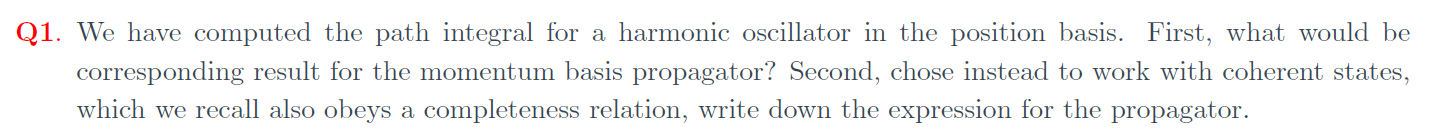
\includegraphics[width=0.85\pagewidth]{1.png}
%%%%%%%%%%%%%%%%%%%%%%
The path integral, or propagator, for the harmonic oscillator was derived in class to be
\begin{equation}
\braket{x_f,t_f}{x_i,t_i}=\sqrt{\frac{m\omega}{2\pi i \sin{\omega T}}}\exp[\frac{i m \omega}{2 }\frac{(x_i^2+x_f^2)\cos{\omega T}-2x_i x_f}{\sin{\omega T}}].
\end{equation}
Note that we have set $\hbar=1$. We will now employ the following trick, which Mukund gave at his office-hour:
\\\\
Since the harmonic oscillator is symmetric in $x$ and $p$, meaning
\begin{equation}
H=\frac{p^2}{2p_0^2}+\frac{x^2}{2x_0^2}
\end{equation}
So any result in the $x$-basis should hold in the $p$-basis under the exchange
\begin{equation}
\frac{p}{p_0}\Leftrightarrow\frac{x}{x_0}
\end{equation}
here $p_0=\sqrt{m}$ and $x_0=\frac{1}{\sqrt{m}\omega}$, so by inspection we have
\begin{equation} \label{eq:p-kernel}
\begin{aligned}
\braket{p_f,t_f}{p_i,t_i}=&\left.	\braket{x_f,t_f}{x_i,t_i}\right|_{x\to p,~~x_0\to p_0}\\
=&\sqrt{\frac{1}{2 \pi i m \omega \sin{\omega T}}}\exp[\frac{i}{2\omega m }\frac{(p_i^2+p_f^2)\cos{\omega T}-2p_i p_f}{\sin{\omega T}}].
\end{aligned}
\end{equation}
Let us explicitly check this, using that we in the previous homework found that the momentum space propagator is related to the positions space propagator through a double Fourier-transform, i.e.
\begin{equation}
\braket{p_f,t_f}{p_i,t_i}=\frac{1}{2\pi}\int\dd x_f \int  \dd x_i \: e^{-ip_fx_f} e^{ip_ix_i} \braket{x_f,t_f}{x_i,t_i}
\end{equation}
Inserting into this, one finds
\begin{equation}
\begin{aligned}
\braket{p_f,t_f}{p_i,t_i}=&\frac{1}{2\pi}\sqrt{\frac{m\omega}{2\pi i \sin{\omega T}}}\int\dd x_f \int  \dd x_i \: e^{-ip_fx_f} e^{ip_ix_i} \exp[\frac{i m \omega}{2 }\frac{(x_i^2+x_f^2)\cos{\omega T}-2x_i x_f}{\sin{\omega T}}]\\
=&\sqrt{\frac{m\omega}{i 8\pi^3 \sin{\omega T}}}\int\dd x_f\int  \dd x_i \: \exp[-ax_i^2+b(x_f)x_i+c(x_f)]
\end{aligned}
\end{equation}
where 
\begin{equation}
\begin{aligned}
a&\equiv-\frac{i}{2}m\omega \cot{T \omega}\\
b(x_f)&\equiv ip_i-im\omega x_f \csc{T\omega}\\
c(x_f)&\equiv\frac{i}{2}m\omega x_f^2 \cot{T\omega}-ip_f x_f
\end{aligned}
\end{equation}
Performing the Gaussian integration we find
\begin{equation}
\begin{aligned}
\braket{p_f,t_f}{p_i,t_i}=&\frac{1}{\sqrt{4\pi^2\cos{\omega T}}}
\int\dd x_f \: \exp[-\frac{i}{2 }
\left(2p_fx_f-2p_ix_f\sec{\omega T}+\left[\frac{p_i^2}{m\omega}+m\omega x_f^2\right]\tan{\omega T}\right)
]\\
=&
\frac{1}{\sqrt{4\pi^2\cos{\omega T}}}
\int\dd x_f \: \exp[-\alpha x_f^2+\beta x_f+\gamma]
\end{aligned}
\end{equation}
where we have collected the constants:
\begin{equation}
\begin{aligned}
\alpha&\equiv\frac{i}{2}m\omega \tan{\omega T}\\
\beta&\equiv ip_i\sec{\omega T} -ip_f\\
\gamma&\equiv \frac{ip_i^2\tan{\omega T}}{2m\omega}
\end{aligned}
\end{equation}
Once again, performing the Gaussian integration we find
\begin{equation}
	\begin{aligned}
		\braket{p_f,t_f}{p_i,t_i}=&\sqrt{\frac{1}{2\pi im\omega \sin{\omega T}}}\exp[\frac{i}{2m\omega}\left(p_f^2\cot{\omega T}+2p_i^2\csc{2\omega T}-2p_ip_f\csc{\omega T}\right)]\\
		=&
		\sqrt{\frac{1}{2\pi im\omega \sin{\omega T}}}\exp[\frac{i}{2\omega m }\frac{(p_i^2+p_f^2)\cos{\omega T}-2p_i p_f}{\sin{\omega T}}]
	\end{aligned}
\end{equation}
Just like we found in \eqref{eq:p-kernel}.
%%%%%%%%%%%%%%%%%%%%%%%%%%%%%%%
Now to find the coherent state propagator we write
\begin{equation}
\begin{aligned}
K(\zeta_f,t_f;\zeta_i,t_i)&=\braket{\zeta_f,t_f}{\zeta_i,t_i}\\
&=\mel{\zeta_f}{U(t_f,t_i)}{\zeta_i}\\
&=\iint \dd x_i\, \dd x_f \,\braket{\zeta_f}{x_f}\hspace*{-0.2cm}\mel{x_f}{U(t_f,t_i)}{x_i}\hspace*{-0.15cm}\braket{x_i}{\zeta_i}\\
&=\iint \dd x_i\, \dd x_f \,\braket{\zeta_f}{x_f}\braket{x_i}{\zeta_i}K(x_f,t_f;x_i,t_i)
\end{aligned}
\end{equation}
We already have the position space propagator, while the wavefunctions in coherent state basis can be readily looked up in e.g. Shankar (eq (21.1.132)) to be
\begin{equation}
\braket{x}{\zeta}=\left(\frac{m\omega}{\pi}\right)^{1/4}e^{-\zeta ^2/2}e^{-m\omega x^2/2}e^{\sqrt{m\omega} \zeta x}
\end{equation}
so the integration is:
\begin{equation}
	\begin{aligned}
		K(\zeta_f,t_f;\zeta_i,t_i)
		&=\frac{m\omega}{\pi}\sqrt{\frac{1}{2i\sin{\omega T}}}\iint \dd x_i\, \dd x_f \,e^{-[(\zeta_f^*)^2+(\zeta_i) ^2] /2}e^{-m\omega [x_f^2+x_i^2]/2}e^{\sqrt{m\omega} \zeta^*_f x_f}e^{\sqrt{m\omega} \zeta_i x_i}\\
		&\qquad\qquad\times\exp[\frac{i m \omega}{2 }\frac{(x_i^2+x_f^2)\cos{\omega T}-2x_i x_f}{\sin{\omega T}}]
	\end{aligned}
\end{equation}
One could then go on to calculate this by performing the two Gaussian integrals, but there is a more efficient way to obtain the propagator, which comes from noticing that a coherent state remains coherent under time evolution,
\begin{equation}
U(t)\ket{\zeta}=e^{a^\dagger(t) \zeta}\ket{0}=e^{a^\dagger \zeta \exp(-i\omega t)}\ket{0}=e^{a^\dagger \zeta' }\ket{0}=\ket{\zeta'}=\ket{\zeta e^{-i\omega t}}
\end{equation}
where we have used the time evolution of $a^\dagger$, namely $a^\dagger (t)=a^\dagger e^{-i\omega t}$. Using this and the normalization $\braket{\zeta_1}{\zeta_2}=e^{\zeta_1^*\zeta_2}$ we then have
\begin{equation}
\begin{aligned}
K(\zeta_f,t_f;\zeta_i,t_i)&=\mel{\zeta_i}{U(t_f,t_i)}{\zeta_i}\\
&=\braket{\zeta_i}{\zeta_f'}=e^{\zeta_i^*\zeta_f'}=e^{\zeta_i^*\zeta_fe^{-i\omega(t_f-t_i)}}
\end{aligned}
\end{equation}
\newpage
\section*{Problem 2}
\hspace*{-1cm}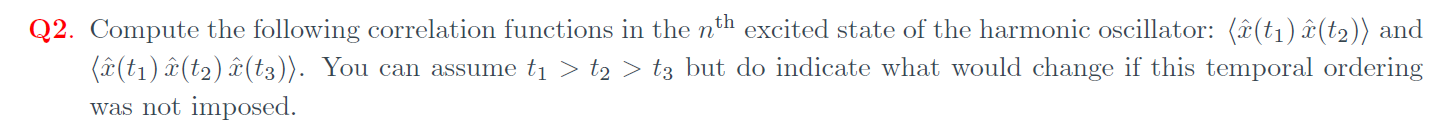
\includegraphics[width=0.85\pagewidth]{2.png}
\underline{Comment about time ordering}. We are calculating a time ordered correlation function and so we if the internal ordering, wasn't consistent with the order $t_1>t_2>t_3$ then we would have to commute the operators through to get the appropriate ordering. 

As an example we could have the time order correlation function $\expval{x(t_2)x(t_1)}=\expval{x(t_1)x(t_2)+[x(t_2),x(t_1)]}$. The commutator is non trivial since these are evaluated at different times, and so the result would deviate from the one we are trying to obtain in this problem.

Now let us note that
%%%%%%%%%%%%%%%%%%%%%%%%%%%%%%%%%%%%%%%%%%
\begin{equation}
	\begin{aligned}
		\mel{n}{x}{m}&=\frac{x_0}{\sqrt{2}}\mel{n}{(a+a^\dagger)}{m}\\
		&=\frac{x_0}{\sqrt{2}}\mel{n}{a}{m}+\frac{x_0}{\sqrt{2}}\mel{n}{a^\dagger}{m}\\
		&=\frac{x_0}{\sqrt{2}}\sqrt{m}\braket{n}{m-1}+\frac{x_0}{\sqrt{2}}\sqrt{m+1}\braket{n}{m+1}\\
		&=\frac{x_0}{\sqrt{2}}\sqrt{m}\delta_{n\,(m-1)}+\frac{x_0}{\sqrt{2}}\sqrt{m+1}\delta_{n\,(m+1)}\\
		\Rightarrow\sum_m\mel{n}{x}{m}&=\frac{x_0}{\sqrt{2}}\sqrt{n+1}+\frac{x_0}{\sqrt{2}}\sqrt{n}
	\end{aligned}
\end{equation}
%%%%%%%%%%%%%%%%%%%%%%%%%%%%%%%%%%%%%%%%%%
Then using this, we can compute the first correlation function
%%%%%%%%%%%%%%%%%%%%%%%%%%%%%%%%%%%%%%%%%%
\begin{equation}
	\begin{aligned}
		\mel{n_1}{x(t_1)x(t_2)}{n_1}=&\mel{n_1}{e^{iHt_1}xe^{iH(t_2-t_1)}xe^{-iHt_2}}{n_1}\\
		=&\sum_{n_2}\mel{n_1}{e^{iHt_1}x\dyad{n_2}{n_2}e^{iH(t_2-t_1)}xe^{-iHt_2}}{n_1}
		\\
		=&\sum_{n_2}e^{iE_{n_1}(t_1-t_2)}e^{iE_{n_2}(t_2-t_1)}\mel{n_1}{x\dyad{n_2}{n_2}x}{n_1}
		\\
		=&\frac{x_0^2}{2}\sum_{n_2} e^{iE_{n_1}(t_1-t_2)}e^{iE_{n_2}(t_2-t_1)}\times \\
		&\left(\sqrt{n_2}\delta_{n_1\,(n_2-1)}+\sqrt{n_2+1}\delta_{n_1\,(n_2+1)}\right)\left(\sqrt{n_2}\delta_{n_1\,(n_2-1)}+\sqrt{n_2+1}\delta_{n_1 \,(n_2+1)}\right)
		\\
		=&\frac{x_0^2}{2}\left(e^{iE_{n_1}(t_1-t_2)}e^{iE_{n_1+1}(t_2-t_1)}(n_{1}+1)+e^{iE_{n_1}(t_1-t_2)}e^{iE_{n_1-1}(t_2-t_1)}n_1\right)
		\\
		=&\frac{x_0^2}{2}\left(e^{i\omega(n_1+\frac{1}{2})(t_1-t_2)}e^{i\omega(n_1+\frac{3}{2})(t_2-t_1)}(n_{1}+1)+e^{i\omega(n_1+\frac{1}{2})(t_1-t_2)}e^{i\omega(n_1-\frac{1}{2})(t_2-t_1)}n_1\right)
		\\
		=&\frac{x_0^2}{2}\left(e^{i\omega(n_1+\frac{1}{2})(t_1-t_2)}e^{i\omega(-n_1-\frac{3}{2})(t_1-t_2)}(n_{1}+1)+e^{i\omega(n_1+\frac{1}{2})(t_1-t_2)}e^{i\omega(-n_1+\frac{1}{2})(t_1-t_2)}n_1\right)
		\\
		=&\frac{x_0^2}{2}\left(e^{-i\omega(t_1-t_2)}(n_{1}+1)+e^{i\omega(t_1-t_2)}n_1\right)
	\\
	=&\frac{x_0^2}{2}n_{1}\left(e^{-i\omega(t_1-t_2)}+e^{i\omega(t_1-t_2)}\right)+\frac{x_0^2}{2}e^{-i\omega(t_1-t_2)}
		\\
	=&\frac{x_0^2}{2}\left(2n_1\cos{\omega (t_1-t_2)}+e^{-i\omega(t_1-t_2)}\right)
	\end{aligned}
\end{equation}
%%%%%%%%%%%%%%%%%%%%%%%%%%%%%%%%%%%%%%%%%%
Also
%%%%%%%%%%%%%%%%%%%%%%%%%%%%%%%%%%%%%%%%%%
\begin{equation}
\begin{aligned}
&\mel{n_1}{x(t_1)x(t_2)x(t_3)}{n_1}\\
=&\mel{n}{e^{iHt_1}xe^{iH(t_2-t_1)}xe^{iH(t_3-t_2)}xe^{-iHt_3}}{n_1}\\
=&\sum_{n_2}\sum_{n_3}\mel{n_1}{e^{iHt_1}x\dyad{n_2}{n_2}e^{iH(t_2-t_1)}xe^{iH(t_3-t_2)}\dyad{n_3}{n_3}xe^{-iHt_3}}{n_1}
\\
=&\sum_{n_2}\sum_{n_3}\underbrace{e^{iE_{n_1}(t_1-t_3)}e^{iE_{n_2}(t_2-t_1)}e^{iE_{n_3}(t_3-t_2)}}_{F(n_1,n_2,n_3)}\mel{n_1}{x\dyad{n_2}{n_2}x\dyad{n_3}{n_3}x}{n_1}
\\
=&\frac{x_0^3}{2^{3/2}}\sum_{n_2}\sum_{n_3}F(n_1,n_2,n_3)\left(\sqrt{n_2}\,\delta_{n_1\,(n_2-1)}+\sqrt{n_2+1}\,\delta_{n_1\,(n_2+1)}\right)\mel{n_2}{x}{n_3}\left(\sqrt{n_3}\,\delta_{n_1\,(n_3-1)}+\sqrt{n_3+1}\,\delta_{n_1\,(n_3+1)}\right)\\
\propto&\mel{n_2}{x}{n_2}\\
=&0
\end{aligned}
\end{equation}
%%%%%%%%%%%%%%
where we in the second to last line have summed over the delta-functions, and we see that the only contributing term vanishes.
\newpage
%%%%%%%%%%%%%%%%%%%%%%%%%%%%%%%%%%%%%%%%%%%%%%%%%%%%%%%%
\section*{Problem 3}
First we recalculate problem 2 for off-diagonal elements, i.e. $\mel{n}{x(t_1)x(t_2)}{m}$. We find
\begin{equation}
	\begin{aligned}
		\mel{n_1}{x(t_1)x(t_2)}{n_4}=&\mel{n}{e^{iHt_1}xe^{iH(t_2-t_1)}xe^{-iHt_2}}{n_4}\\
		=&\sum_{n_2}\mel{n_1}{e^{iHt_1}x\dyad{n_2}{n_2}e^{iH(t_2-t_1)}xe^{-iHt_2}}{n_4}
		\\
		=&\sum_{n_2} e^{i(E_{n_1}-E_{n_2})t_1}e^{i(E_{n_2}-E_{n_4})t_2}\mel{n_1}{x\dyad{n_2}{n_2}x}{n_4}
		\\
		=&\frac{x_0}{2}\sum_{n_2} e^{i(E_{n_1}-E_{n_2})t_1}e^{i(E_{n_2}-E_{n_4})t_2}\times \\
		&\left(\sqrt{n_2}\delta_{n_1\,(n_2-1)}+\sqrt{n_2+1}\delta_{n_1\,(n_2+1)}\right)\left(\sqrt{n_2}\delta_{n_4\,(n_2-1)}+\sqrt{n_2+1}\delta_{n_4\,(n_2+1)}\right)
		\\
		=&\frac{x_0}{2}\sum_{n_2} e^{i(E_{n_1}-E_{n_2})t_1}e^{i(E_{n_2}-E_{n_4})t_2}\times \\
		&\left(\sqrt{n_2}\delta_{(n_1+1)\,n_2}\sqrt{n_2}\delta_{(n_4+1)\,(n_2)}+\sqrt{n_2+1}\delta_{(n_1-1)\,n_2}\sqrt{n_2}\delta_{(n_4+1)\,(n_2)}\right.\\
		&\quad+\sqrt{n_2}\delta_{(n_1+1)\,n_2}\sqrt{n_2+1}\delta_{(n_4-1)\,(n_2)}+\left.\sqrt{n_2+1}\delta_{(n_1-1)\,n_2}\sqrt{n_2+1}\delta_{(n_4-1)\,(n_2)}\right)
		\\
	=&\frac{x_0}{2} e^{i(E_{n_1}-E_{n_1+1})t_1}e^{i(E_{n_4+1}-E_{n_4})t_2}(n_1+1)\delta_{n_1\,n_4}\\
	&+\frac{x_0}{2} e^{i(E_{n_1}-E_{n_1-1})t_1}e^{i(E_{n_4+1}-E_{n_4})t_2}\sqrt{(n_1-1)n_1}\delta_{n_1\,(n_4+2)}\\
	&+\frac{x_0}{2} e^{i(E_{n_1}-E_{n_1-1})t_1}e^{i(E_{n_4-1}-E_{n_4})t_2} \sqrt{(n+1)(n_1+2)}\delta_{n_1\,n_4-2}\\
	&+\frac{x_0}{2} e^{i(E_{n_1}-E_{n_1-1})t_1}e^{i(E_{n_4-1}-E_{n_4})t_2}n_1\delta_{n_1\,n_4}
		\\
=&\frac{x_0^2}{2}\left( e^{-i\omega (t_1-t_2)}(n_1+1)\delta_{n_1\,n_4}+ e^{i \omega (t_1+t_2)}\sqrt{(n_4+1)n_1}\delta_{n_1\,(n_4+2)}\right.\\
&\left.+ e^{-i\omega (t_1+t_2)}\sqrt{(n+1)(n_4)}\delta_{n_1\,(n_4-2)}+ e^{i\omega (t_1-t_2)}n_1\delta_{n_1\,n_4}\right)\\
	\end{aligned}
\end{equation}
The diagonal elements here reduce to the same ones we found in problem 2, i.e. we expect this to hold.
%%
Also the coherent states have the following property, see e.g Shankar.
\begin{equation}
\begin{aligned}
\braket{\zeta}{n}&=\frac{(\zeta^*)^n}{\sqrt{n!}}\\
\braket{n}{\zeta}&=\frac{\zeta^n}{\sqrt{n!}}\\
\end{aligned}
\end{equation}
We then compute  $\mel{\zeta}{x(t_1)x(t_2)}{\zeta}$ by inserting two othonormal basis sets and using the just derived results for $\mel{n}{x(t_1)x(t_2)}{m}$.
%%%%%%%%%%%%%%%%%%%%%%%%%%%%%%%%%%%%%%%%%%%
\begin{equation}
	\begin{aligned}
		\mel{\zeta}{x(t_1)x(t_2)}{\zeta}=&\sum_{\substack{n_1\\n_4}}\braket{\zeta}{n_1}\hspace*{-0.2cm}\mel{n_1}{x(t_1)x(t_2)}{n_4}\hspace*{-0.15cm}\braket{n_4}{\zeta}
		\\
=&\frac{x_0^2}{2}\sum_{\substack{n_1\\n_4}}\frac{(\zeta^*)^{n_1}\zeta^{n_4}}{\sqrt{n_1!n_4!}}\left(  e^{-i\omega (t_1-t_2)}(n_1+1)\delta_{n_1\,n_4}\right.\\
&\qquad\qquad+ e^{i \omega (t_1+t_2)}\sqrt{(n_4+1)n_1}\delta_{n_1\,(n_4+2)}\\
&\qquad\qquad+ e^{-i\omega (t_1+t_2)}\sqrt{(n_1+1)n_4}\delta_{n_1\,(n_4-2)}\\
&\qquad\qquad+ \left.e^{i\omega (t_1-t_2)}n_1\delta_{n_1\,n_4}\right)
		\\
=&\frac{x_0^2}{2}\sum_{\substack{n_1}}\frac{|\zeta|^{2n_1}}{n_1!}\left(  e^{-i\omega (t_1-t_2)}(n_1+1)+e^{i\omega (t_1-t_2)}n_1\right)\\
+&\frac{x_0^2}{2}\sum_{\substack{n_1\\ n_4}}\frac{(\zeta^*)^{n_1}\zeta^{n_4}}{(\sqrt{n_1!}\sqrt{n_4!}}\left( e^{-i\omega (t_1+t_2)}\sqrt{(n_1+1)n_4}\delta_{n_1\,(n_4-2)}\right)\\
+&\frac{x_0^2}{2}\sum_{\substack{n_1\\ n_4}}\frac{(\zeta^*)^{n_1}\zeta^{n_4}}{(\sqrt{n_1!}\sqrt{n_4!}}\left(  e^{i \omega (t_1+t_2)}\sqrt{(n_4+1)n_1}\delta_{(n_1-2)\,n_4}\right)
	\end{aligned}
\end{equation}
Then using
\begin{equation}
\begin{aligned}
\sum_{n}\frac{(x^2)^n}{n!}n&=x^2e^{x^2}\\
\sum_n\frac{(x^2)^n}{n!}&=e^{x^2},
\end{aligned}
\end{equation}
and summing over the deltafunctions, we find
\begin{equation}
	\begin{aligned}
		\mel{\zeta}{x(t_1)x(t_2)}{\zeta}
		=&\frac{x_0^2}{2}e^{|\zeta|^2}\left((|\zeta|^{2}+1)e^{-i\omega (t_1-t_2)}+|\zeta|^2 e^{i\omega (t_1-t_2)}\right)\\
		&+\frac{x_0^2}{2}e^{|\zeta|^2}\left(\zeta^2 e^{-i\omega (t_1+t_2)}\right)\\
	&+\frac{x_0^2}{2}e^{|\zeta|^2}\left((\zeta^*)^2 e^{i\omega (t_1+t_2)}\right)\\
	=&\frac{x_0^2}{2}e^{|\zeta|^2}\left(2|\zeta|^{2}\cosh[i\omega(t_1-t_2)]+e^{-i\omega (t_1+t_2)}\right)\\
	&+x_0^2e^{|\zeta|^2}\Re[\zeta^2 e^{-i\omega (t_1+t_2)}]\\
		=&\frac{x_0^2}{2}e^{|\zeta|^2}\left(2|\zeta|^{2}\cosh[i\omega(t_1-t_2)]+e^{-i\omega (t_1+t_2)}+2\Re[\zeta^2]\cos{\omega (t_1+t_2)}\right)
	\end{aligned}
\end{equation}
%%%%%%%%%%%%%%%%%%%%%%%%%%%%%%%%%%%%%%%%%%%
For the second part of the problem:
\begin{equation}
\begin{aligned}
\Tr(e^{-\beta H}x(t_1)x(t_2))&=\sum_n \mel{n}{e^{-\beta H}x(t_1)x(t_2)}{n}\\
&=\sum_ne^{-\beta E_n} \mel{n}{x(t_1)x(t_2)}{n}\\
&=\sum_ne^{-\beta\omega (n+\frac{1}{2})}\frac{x_0^2}{2}\left(2n_1\cos{\omega (t_1-t_2)}+e^{-i\omega(t_1-t_2)}\right)\\
&=x_0^2\cos{\omega (t_1-t_2)}\sum_ne^{-\beta\omega (n+\frac{1}{2})}n_1+\frac{x_0^2}{2}e^{-i\omega(t_1-t_2)}\sum_ne^{-\beta\omega(n+\frac{1}{2})}\\
\end{aligned}
\end{equation}
Then using
\begin{equation}
	\begin{aligned}
		\sum_{n}e^{-k(n+\frac{1}{2})}=&\frac{e^{k/2}}{e^{k}-1}\\
		\sum_{n}e^{-k(n+\frac{1}{2})}n=&\frac{e^{k/2}}{\left(e^{k}-1\right)^2}
	\end{aligned}
\end{equation}
%%%%%%%%%%%%%%%%%%%%%%%%%%%%%%%%%%%%%%%%%%
we find
\begin{equation}
	\begin{aligned}
		\Tr(e^{-\beta H}x(t_1)x(t_2))&=\sum_n \mel{n}{e^{-\beta H}x(t_1)x(t_2)}{n}\\
		&=x_0^2\cos{\omega (t_1-t_2)}\frac{e^{\beta \omega /2}}{\left(e^{\beta \omega }-1\right)^2}+\frac{x_0^2}{2}e^{-i\omega(t_1-t_2)}\frac{e^{\beta \omega /2}}{\left(e^{\beta \omega }-1\right)}
		\\
		&=\frac{1}{4} x_0^2 \csch\left(\frac{\beta\omega}{2}\right) \left(\cos{\omega (t_1-t_2)} \left[\coth \left(\frac{\beta\omega}{2}\right)-1\right]+e^{-i\omega(t_1-t_2)}\right)
	\end{aligned}
\end{equation}
Where we have converted to hyperbolic functions in the last line in the last line.
\newpage
\section*{Problem 4}
\underline{Note:} There are many approaches than can be taken in this problem. Since I have solved it before in a previous QM class (see problem 5.4.3 in Shankar), I will do the problem in the same manor I have done previously and not the way it was discussed at the office hour. The results obtained matches the ones asked for, by Shankar and so should be correct.\\\\
We have the following Hamiltonian
\be
\ham=\kin+fx
\ee
And we have to find the propagator given by
\be
K(x,t|x',t=0)=\mel{x}{e^{-\frac{i}{\hbar}\ham (t-t')}}{x'}
\ee
Since our Hamiltonians dependence on $x$ is simpler than it's dependence on $p$ it would instead be easier to calculate the propagator in the momentum bases and then transfer to position space afterwards:
\[
K(x,t|x',0)=\frac{1}{2\pi}\int^{\infty}_{-\infty}\dd p\int^{\infty}_{-\infty}\dd p'\: K(p,t|p',0)e^{\frac{i}{\hbar}px}e^{\frac{i}{\hbar}p'x'}
\]
Where we have set $\hbar=1$. We first have to obtain the initial states. We first write the Schrödinger equation for stationary states:
\be
\ham\ket{\psi}=E\ket{\psi}
\ee
in the momentum basis where we have the operator $\hat{x}=i\pdv{}{p}$ this is just:
\be
\left(\frac{p^2}{2m}+if \pdv{}{p}\right)\psi(p)=E\psi(p)
\ee
Rearranging the terms we get:
\[
\pdv{\psi(p)}{p}= \underbrace{\left[\left( E-\frac{p^2}{2m} \right)\frac{i}{\hbar f}\right]}_{=\text{function of } p}\psi(p)
\]
The solution to this is just the exponential function:
\[
\psi(p)=C\exp[\frac{i}{\hbar f}\left( E-\frac{p^2}{6m} \right)p]
\]
The constant $C$ can be found from the normalization condition
\be
\braket{\psi_E(p)}{\psi_{E'}(p)}=\delta(E-E')
\ee
We have
\[
|C|^2\int^{\infty}_{-\infty}\dd p\:\exp[\frac{i}{\hbar f}\left( E-E' \right)p]
=|C|^22\pi\hbar f\delta(E-E')\Rightarrow |C|^2=\frac{1}{2\pi\hbar f}
\]
Where we have used the following property of the dirac delta function:
\[
\delta(x-x')=\frac{1}{2\pi}\int^{\infty}_{-\infty}e^{i(x-x')p}\:\dd p
\]
We can now find the propagator in the momentum basis
\[
K(p,t|p',0)=\frac{1}{2\pi f}\int^{\infty}_{-\infty}\dd E \exp[\frac{i}{ f}\left( Ep-\frac{p^3}{6m} \right)]\exp[-\frac{i}{ f}\left( Ep'-\frac{p'^3}{6m} \right)]\exp[-iE(t-t')]
\]
\[
K(p,t|p',0)=\frac{1}{2\pi f}\int^{\infty}_{-\infty}\dd E \exp[\frac{i}{ f}E\left( p-p'-f(t-t') \right)]\exp[\frac{i}{ f}\frac{p'^3-p^3}{6m}]
\]
Again using the fact that this just integrates out to the Dirac Delta function we get:
\[
K(p,t|p',0)=\delta (p-p'-f(t-t'))\exp[\frac{i}{f}\frac{p'^3-p^3}{6m}]
\]
We can now obtain the propagator in position space
\[
K(x,t|x',0)=\frac{1}{2\pi}\int^{\infty}_{-\infty}\dd p\int^{\infty}_{-\infty}\dd p'\:\delta (p-p'-f(t-t'))\exp[\frac{i}{ f}\frac{p'^3-p^3}{6m}]\exp[ipx]\exp[ip'x'
]
\]
Integrating over the deltafunction gives
\[
K(x,t|x',0)=\frac{1}{2\pi}\int^{\infty}_{-\infty}\dd p\:\exp[\frac{i}{ f}\frac{(p-f(t-t'))^3-p^3}{6m}]\exp[\frac{i}{\hbar}px]\exp[\frac{i}{\hbar}(p-f(t-t'))x'
]
\]
plugging this integral into Mathematica and simplifying we get:
\[
K(x,t|x',0)=\sqrt{\frac{m}{2\pi i (t-t')}}\exp[i\left( \frac{m(x-x')^2}{2(t-t')}-\frac{1}{2}f(t-t')(x-x')-\frac{1}{24m}f^2(t-t')^2 \right)]
\]
\end{document}

